% Created by tikzDevice version 0.12.3 on 2020-04-10 11:40:59
% !TEX encoding = UTF-8 Unicode
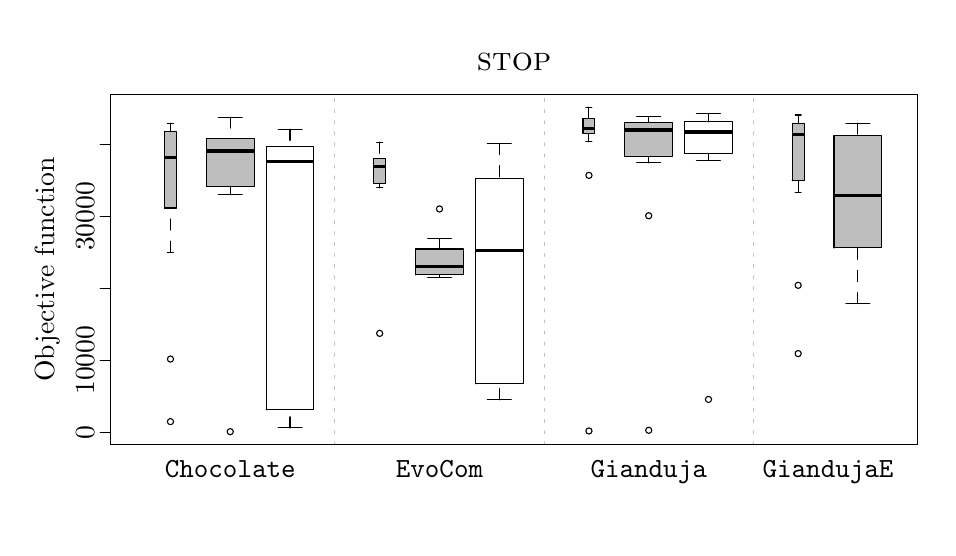
\begin{tikzpicture}[x=1pt,y=1pt]
\definecolor{fillColor}{RGB}{255,255,255}
\path[use as bounding box,fill=fillColor,fill opacity=0.00] (0,0) rectangle (325.21,180.67);
\begin{scope}
\path[clip] ( 30.00, 30.00) rectangle (321.61,156.67);
\definecolor{fillColor}{RGB}{190,190,190}

\path[fill=fillColor] ( 49.44,115.52) --
	( 53.76,115.52) --
	( 53.76,143.04) --
	( 49.44,143.04) --
	cycle;
\definecolor{drawColor}{RGB}{0,0,0}

\path[draw=drawColor,line width= 1.2pt,line join=round] ( 49.44,133.75) -- ( 53.76,133.75);

\path[draw=drawColor,line width= 0.4pt,dash pattern=on 4pt off 4pt ,line join=round,line cap=round] ( 51.60, 99.56) -- ( 51.60,115.52);

\path[draw=drawColor,line width= 0.4pt,dash pattern=on 4pt off 4pt ,line join=round,line cap=round] ( 51.60,146.15) -- ( 51.60,143.04);

\path[draw=drawColor,line width= 0.4pt,line join=round,line cap=round] ( 50.52, 99.56) -- ( 52.68, 99.56);

\path[draw=drawColor,line width= 0.4pt,line join=round,line cap=round] ( 50.52,146.15) -- ( 52.68,146.15);

\path[draw=drawColor,line width= 0.4pt,line join=round,line cap=round] ( 49.44,115.52) --
	( 53.76,115.52) --
	( 53.76,143.04) --
	( 49.44,143.04) --
	( 49.44,115.52);

\path[draw=drawColor,line width= 0.4pt,line join=round,line cap=round] ( 51.60, 60.93) circle (  1.12);

\path[draw=drawColor,line width= 0.4pt,line join=round,line cap=round] ( 51.60, 38.31) circle (  1.12);

\path[fill=fillColor] ( 64.56,123.37) --
	( 81.84,123.37) --
	( 81.84,140.78) --
	( 64.56,140.78) --
	cycle;

\path[draw=drawColor,line width= 1.2pt,line join=round] ( 64.56,136.16) -- ( 81.84,136.16);

\path[draw=drawColor,line width= 0.4pt,dash pattern=on 4pt off 4pt ,line join=round,line cap=round] ( 73.20,120.29) -- ( 73.20,123.37);

\path[draw=drawColor,line width= 0.4pt,dash pattern=on 4pt off 4pt ,line join=round,line cap=round] ( 73.20,148.35) -- ( 73.20,140.78);

\path[draw=drawColor,line width= 0.4pt,line join=round,line cap=round] ( 68.88,120.29) -- ( 77.52,120.29);

\path[draw=drawColor,line width= 0.4pt,line join=round,line cap=round] ( 68.88,148.35) -- ( 77.52,148.35);

\path[draw=drawColor,line width= 0.4pt,line join=round,line cap=round] ( 64.56,123.37) --
	( 81.84,123.37) --
	( 81.84,140.78) --
	( 64.56,140.78) --
	( 64.56,123.37);

\path[draw=drawColor,line width= 0.4pt,line join=round,line cap=round] ( 73.20, 34.69) circle (  1.12);
\definecolor{fillColor}{RGB}{255,255,255}

\path[fill=fillColor] ( 86.16, 42.59) --
	(103.44, 42.59) --
	(103.44,137.61) --
	( 86.16,137.61) --
	cycle;

\path[draw=drawColor,line width= 1.2pt,line join=round] ( 86.16,132.27) -- (103.44,132.27);

\path[draw=drawColor,line width= 0.4pt,dash pattern=on 4pt off 4pt ,line join=round,line cap=round] ( 94.80, 36.05) -- ( 94.80, 42.59);

\path[draw=drawColor,line width= 0.4pt,dash pattern=on 4pt off 4pt ,line join=round,line cap=round] ( 94.80,143.97) -- ( 94.80,137.61);

\path[draw=drawColor,line width= 0.4pt,line join=round,line cap=round] ( 90.48, 36.05) -- ( 99.12, 36.05);

\path[draw=drawColor,line width= 0.4pt,line join=round,line cap=round] ( 90.48,143.97) -- ( 99.12,143.97);

\path[draw=drawColor,line width= 0.4pt,line join=round,line cap=round] ( 86.16, 42.59) --
	(103.44, 42.59) --
	(103.44,137.61) --
	( 86.16,137.61) --
	( 86.16, 42.59);
\definecolor{fillColor}{RGB}{190,190,190}

\path[fill=fillColor] (125.04,124.44) --
	(129.37,124.44) --
	(129.37,133.29) --
	(125.04,133.29) --
	cycle;

\path[draw=drawColor,line width= 1.2pt,line join=round] (125.04,130.43) -- (129.37,130.43);

\path[draw=drawColor,line width= 0.4pt,dash pattern=on 4pt off 4pt ,line join=round,line cap=round] (127.20,122.81) -- (127.20,124.44);

\path[draw=drawColor,line width= 0.4pt,dash pattern=on 4pt off 4pt ,line join=round,line cap=round] (127.20,139.29) -- (127.20,133.29);

\path[draw=drawColor,line width= 0.4pt,line join=round,line cap=round] (126.12,122.81) -- (128.29,122.81);

\path[draw=drawColor,line width= 0.4pt,line join=round,line cap=round] (126.12,139.29) -- (128.29,139.29);

\path[draw=drawColor,line width= 0.4pt,line join=round,line cap=round] (125.04,124.44) --
	(129.37,124.44) --
	(129.37,133.29) --
	(125.04,133.29) --
	(125.04,124.44);

\path[draw=drawColor,line width= 0.4pt,line join=round,line cap=round] (127.20, 70.21) circle (  1.12);

\path[fill=fillColor] (140.17, 91.38) --
	(157.45, 91.38) --
	(157.45,100.69) --
	(140.17,100.69) --
	cycle;

\path[draw=drawColor,line width= 1.2pt,line join=round] (140.17, 94.39) -- (157.45, 94.39);

\path[draw=drawColor,line width= 0.4pt,dash pattern=on 4pt off 4pt ,line join=round,line cap=round] (148.81, 90.45) -- (148.81, 91.38);

\path[draw=drawColor,line width= 0.4pt,dash pattern=on 4pt off 4pt ,line join=round,line cap=round] (148.81,104.35) -- (148.81,100.69);

\path[draw=drawColor,line width= 0.4pt,line join=round,line cap=round] (144.49, 90.45) -- (153.13, 90.45);

\path[draw=drawColor,line width= 0.4pt,line join=round,line cap=round] (144.49,104.35) -- (153.13,104.35);

\path[draw=drawColor,line width= 0.4pt,line join=round,line cap=round] (140.17, 91.38) --
	(157.45, 91.38) --
	(157.45,100.69) --
	(140.17,100.69) --
	(140.17, 91.38);

\path[draw=drawColor,line width= 0.4pt,line join=round,line cap=round] (148.81,115.16) circle (  1.12);
\definecolor{fillColor}{RGB}{255,255,255}

\path[fill=fillColor] (161.77, 52.01) --
	(179.05, 52.01) --
	(179.05,126.18) --
	(161.77,126.18) --
	cycle;

\path[draw=drawColor,line width= 1.2pt,line join=round] (161.77,100.25) -- (179.05,100.25);

\path[draw=drawColor,line width= 0.4pt,dash pattern=on 4pt off 4pt ,line join=round,line cap=round] (170.41, 46.19) -- (170.41, 52.01);

\path[draw=drawColor,line width= 0.4pt,dash pattern=on 4pt off 4pt ,line join=round,line cap=round] (170.41,138.78) -- (170.41,126.18);

\path[draw=drawColor,line width= 0.4pt,line join=round,line cap=round] (166.09, 46.19) -- (174.73, 46.19);

\path[draw=drawColor,line width= 0.4pt,line join=round,line cap=round] (166.09,138.78) -- (174.73,138.78);

\path[draw=drawColor,line width= 0.4pt,line join=round,line cap=round] (161.77, 52.01) --
	(179.05, 52.01) --
	(179.05,126.18) --
	(161.77,126.18) --
	(161.77, 52.01);
\definecolor{fillColor}{RGB}{190,190,190}

\path[fill=fillColor] (200.65,142.49) --
	(204.97,142.49) --
	(204.97,148.00) --
	(200.65,148.00) --
	cycle;

\path[draw=drawColor,line width= 1.2pt,line join=round] (200.65,144.28) -- (204.97,144.28);

\path[draw=drawColor,line width= 0.4pt,dash pattern=on 4pt off 4pt ,line join=round,line cap=round] (202.81,139.41) -- (202.81,142.49);

\path[draw=drawColor,line width= 0.4pt,dash pattern=on 4pt off 4pt ,line join=round,line cap=round] (202.81,151.98) -- (202.81,148.00);

\path[draw=drawColor,line width= 0.4pt,line join=round,line cap=round] (201.73,139.41) -- (203.89,139.41);

\path[draw=drawColor,line width= 0.4pt,line join=round,line cap=round] (201.73,151.98) -- (203.89,151.98);

\path[draw=drawColor,line width= 0.4pt,line join=round,line cap=round] (200.65,142.49) --
	(204.97,142.49) --
	(204.97,148.00) --
	(200.65,148.00) --
	(200.65,142.49);

\path[draw=drawColor,line width= 0.4pt,line join=round,line cap=round] (202.81,127.30) circle (  1.12);

\path[draw=drawColor,line width= 0.4pt,line join=round,line cap=round] (202.81, 34.94) circle (  1.12);

\path[fill=fillColor] (215.77,134.06) --
	(233.05,134.06) --
	(233.05,146.38) --
	(215.77,146.38) --
	cycle;

\path[draw=drawColor,line width= 1.2pt,line join=round] (215.77,143.66) -- (233.05,143.66);

\path[draw=drawColor,line width= 0.4pt,dash pattern=on 4pt off 4pt ,line join=round,line cap=round] (224.41,131.84) -- (224.41,134.06);

\path[draw=drawColor,line width= 0.4pt,dash pattern=on 4pt off 4pt ,line join=round,line cap=round] (224.41,148.57) -- (224.41,146.38);

\path[draw=drawColor,line width= 0.4pt,line join=round,line cap=round] (220.09,131.84) -- (228.73,131.84);

\path[draw=drawColor,line width= 0.4pt,line join=round,line cap=round] (220.09,148.57) -- (228.73,148.57);

\path[draw=drawColor,line width= 0.4pt,line join=round,line cap=round] (215.77,134.06) --
	(233.05,134.06) --
	(233.05,146.38) --
	(215.77,146.38) --
	(215.77,134.06);

\path[draw=drawColor,line width= 0.4pt,line join=round,line cap=round] (224.41,112.71) circle (  1.12);

\path[draw=drawColor,line width= 0.4pt,line join=round,line cap=round] (224.41, 35.17) circle (  1.12);
\definecolor{fillColor}{RGB}{255,255,255}

\path[fill=fillColor] (237.37,135.17) --
	(254.65,135.17) --
	(254.65,146.65) --
	(237.37,146.65) --
	cycle;

\path[draw=drawColor,line width= 1.2pt,line join=round] (237.37,142.93) -- (254.65,142.93);

\path[draw=drawColor,line width= 0.4pt,dash pattern=on 4pt off 4pt ,line join=round,line cap=round] (246.01,132.77) -- (246.01,135.17);

\path[draw=drawColor,line width= 0.4pt,dash pattern=on 4pt off 4pt ,line join=round,line cap=round] (246.01,149.64) -- (246.01,146.65);

\path[draw=drawColor,line width= 0.4pt,line join=round,line cap=round] (241.69,132.77) -- (250.33,132.77);

\path[draw=drawColor,line width= 0.4pt,line join=round,line cap=round] (241.69,149.64) -- (250.33,149.64);

\path[draw=drawColor,line width= 0.4pt,line join=round,line cap=round] (237.37,135.17) --
	(254.65,135.17) --
	(254.65,146.65) --
	(237.37,146.65) --
	(237.37,135.17);

\path[draw=drawColor,line width= 0.4pt,line join=round,line cap=round] (246.01, 46.34) circle (  1.12);
\definecolor{fillColor}{RGB}{190,190,190}

\path[fill=fillColor] (276.25,125.29) --
	(280.57,125.29) --
	(280.57,145.96) --
	(276.25,145.96) --
	cycle;

\path[draw=drawColor,line width= 1.2pt,line join=round] (276.25,141.97) -- (280.57,141.97);

\path[draw=drawColor,line width= 0.4pt,dash pattern=on 4pt off 4pt ,line join=round,line cap=round] (278.41,121.22) -- (278.41,125.29);

\path[draw=drawColor,line width= 0.4pt,dash pattern=on 4pt off 4pt ,line join=round,line cap=round] (278.41,149.11) -- (278.41,145.96);

\path[draw=drawColor,line width= 0.4pt,line join=round,line cap=round] (277.33,121.22) -- (279.49,121.22);

\path[draw=drawColor,line width= 0.4pt,line join=round,line cap=round] (277.33,149.11) -- (279.49,149.11);

\path[draw=drawColor,line width= 0.4pt,line join=round,line cap=round] (276.25,125.29) --
	(280.57,125.29) --
	(280.57,145.96) --
	(276.25,145.96) --
	(276.25,125.29);

\path[draw=drawColor,line width= 0.4pt,line join=round,line cap=round] (278.41, 62.90) circle (  1.12);

\path[draw=drawColor,line width= 0.4pt,line join=round,line cap=round] (278.41, 87.57) circle (  1.12);

\path[fill=fillColor] (291.37,101.10) --
	(308.65,101.10) --
	(308.65,141.66) --
	(291.37,141.66) --
	cycle;

\path[draw=drawColor,line width= 1.2pt,line join=round] (291.37,120.10) -- (308.65,120.10);

\path[draw=drawColor,line width= 0.4pt,dash pattern=on 4pt off 4pt ,line join=round,line cap=round] (300.01, 80.93) -- (300.01,101.10);

\path[draw=drawColor,line width= 0.4pt,dash pattern=on 4pt off 4pt ,line join=round,line cap=round] (300.01,146.18) -- (300.01,141.66);

\path[draw=drawColor,line width= 0.4pt,line join=round,line cap=round] (295.69, 80.93) -- (304.33, 80.93);

\path[draw=drawColor,line width= 0.4pt,line join=round,line cap=round] (295.69,146.18) -- (304.33,146.18);

\path[draw=drawColor,line width= 0.4pt,line join=round,line cap=round] (291.37,101.10) --
	(308.65,101.10) --
	(308.65,141.66) --
	(291.37,141.66) --
	(291.37,101.10);
\definecolor{drawColor}{RGB}{190,190,190}

\path[draw=drawColor,line width= 0.4pt,dash pattern=on 1pt off 3pt ,line join=round,line cap=round] (111.00, 30.00) -- (111.00,156.67);

\path[draw=drawColor,line width= 0.4pt,dash pattern=on 1pt off 3pt ,line join=round,line cap=round] (186.61, 30.00) -- (186.61,156.67);

\path[draw=drawColor,line width= 0.4pt,dash pattern=on 1pt off 3pt ,line join=round,line cap=round] (262.21, 30.00) -- (262.21,156.67);
\end{scope}
\begin{scope}
\path[clip] (  0.00,  0.00) rectangle (325.21,180.67);
\definecolor{drawColor}{RGB}{0,0,0}

\node[text=drawColor,anchor=base,inner sep=0pt, outer sep=0pt, scale=  1.00] at ( 73.20, 18.00) {\texttt{Chocolate}};

\node[text=drawColor,anchor=base,inner sep=0pt, outer sep=0pt, scale=  1.00] at (148.81, 18.00) {\texttt{EvoCom}};

\node[text=drawColor,anchor=base,inner sep=0pt, outer sep=0pt, scale=  1.00] at (224.41, 18.00) {\texttt{Gianduja}};

\node[text=drawColor,anchor=base,inner sep=0pt, outer sep=0pt, scale=  1.00] at (289.21, 18.00) {\texttt{GiandujaE}};
\end{scope}
\begin{scope}
\path[clip] (  0.00,  0.00) rectangle (325.21,180.67);
\definecolor{drawColor}{RGB}{0,0,0}

\node[text=drawColor,anchor=base,inner sep=0pt, outer sep=0pt, scale=  1.20] at (175.81,165.07) {\textsc{stop}};

\node[text=drawColor,rotate= 90.00,anchor=base,inner sep=0pt, outer sep=0pt, scale=  1.00] at (  9.60, 93.34) {Objective function};
\end{scope}
\begin{scope}
\path[clip] (  0.00,  0.00) rectangle (325.21,180.67);
\definecolor{drawColor}{RGB}{0,0,0}

\path[draw=drawColor,line width= 0.4pt,line join=round,line cap=round] ( 30.00, 34.53) -- ( 30.00,138.51);

\path[draw=drawColor,line width= 0.4pt,line join=round,line cap=round] ( 30.00, 34.53) -- ( 26.20, 34.53);

\path[draw=drawColor,line width= 0.4pt,line join=round,line cap=round] ( 30.00, 60.52) -- ( 26.20, 60.52);

\path[draw=drawColor,line width= 0.4pt,line join=round,line cap=round] ( 30.00, 86.52) -- ( 26.20, 86.52);

\path[draw=drawColor,line width= 0.4pt,line join=round,line cap=round] ( 30.00,112.51) -- ( 26.20,112.51);

\path[draw=drawColor,line width= 0.4pt,line join=round,line cap=round] ( 30.00,138.51) -- ( 26.20,138.51);

\node[text=drawColor,rotate= 90.00,anchor=base,inner sep=0pt, outer sep=0pt, scale=  1.00] at ( 24.00, 34.53) {0};

\node[text=drawColor,rotate= 90.00,anchor=base,inner sep=0pt, outer sep=0pt, scale=  1.00] at ( 24.00, 60.52) {10000};

\node[text=drawColor,rotate= 90.00,anchor=base,inner sep=0pt, outer sep=0pt, scale=  1.00] at ( 24.00,112.51) {30000};

\path[draw=drawColor,line width= 0.4pt,line join=round,line cap=round] ( 30.00, 30.00) --
	(321.61, 30.00) --
	(321.61,156.67) --
	( 30.00,156.67) --
	( 30.00, 30.00);
\end{scope}
\end{tikzpicture}
